\documentclass[letterpaper,11pt]{article}

% Soporte para los acentos.
\usepackage[utf8]{inputenc}
\usepackage[T1]{fontenc}
% Idioma español.
\usepackage[spanish,mexico, es-tabla]{babel}
\usepackage{graphicx}
% Modificamos los márgenes del documento.                                       %
\usepackage[lmargin=2cm,rmargin=2cm,top=2cm,bottom=2cm]{geometry}

\title{Facultad de Ciencias, UNAM \\ 
       Reconocimiento de patrones y aprendizaje automatizado \\ 
       Tarea 1: Ensayo inicial}
\author{Rubí Rojas Tania Michelle}
\date{28 de septiembre de 2020}

\begin{document}
\maketitle
¿Qué es aprender? Al momento de escribir estas líneas, aún no tengo clara la 
definición. Aprender es algo que hemos hecho desde pequeños, pero es algo que 
nos cuestionamos muy poco (o en un peor caso, nunca). ¿Cómo puedo saber si 
aprendí algo, o simplemente lo memoricé/mecanicé? La respuesta a esta pregunta 
la encontré hace algunos meses atrás, cuando me encontraba cursando Álgebra 
Moderna II. Como casi no acudía a clases, le pedí a uno de mis amiguitos que 
me apoyara con algunas dudas que tenía sobre Teoría de Galois, pues de eso 
trataría nuestro último examen. Las preguntas de éste saldrían de la tarea 
que nos dejaron unas semanas antes, así que quería resolver la mayor cantidad 
de ejercicios para ir bien preparada. Me llevé una enorme sorpresa cuando mi  
amigo en cuestión sólo podía \textit{pasarme} la demostración, pero no 
explicarme cómo había resuelto el ejercicio. Me dijo que sus otros amigos le 
\textit{rolaban} los ejercicios, y él solo los memorizaba. Es decir, la 
demostración estaba muy bien explicada, pero no podía resolver las dudas que 
yo tenía. Tal vez este ejemplo es muy extremo, pero creo que esto sucede la 
mayoría de las veces durante nuestra educación: simplemente nos limitamos a 
memorizar cosas. Yo misma he sido objeto de dicha barbaridad durante la 
preparatoria, específicamente en mi clase de Psicología. En ese entonces no 
me llamaban mucho la atención los temas que se tocaban, así que prefería 
memorizar las preguntas que vendrían en el examen, y así no preocuparme tanto
por esa materia. Estos recuerdos me vinieron a la mente cuando leí el siguiente
párrafo de \textit{Funes El Memorioso}:
\begin{center}
    \texttt{"Había aprendido sin esfuerzo el inglés, el francés, el portugués, 
    el latín. Sospecho, sin embargo, que no era muy capaz de pensar. Pensar 
    es olvidar diferencias, es generalizar, abstraer. En el abarrotado mundo 
    de Funes no había sino detalles, casi inmediatos."}
\end{center}

Mi memoría no es la mejor. Aunque no sea lo más común, debo admitir que 
escasamente tengo recuerdos de mi vida. Curiosamente, hace un año conocí a un 
chico que presumía de tener memoria fotográfica. Nunca se me ocurrió poner 
a prueba dicha característica, pero me hubiera gustado hacerlo. Antes pensaba
que tener una súper memoria sería todo un don, pero ahora que he leído sobre 
Funes, reconsideré totalmente mis pensamientos. De este hombre me llamó mucho 
la atención el hecho de que él considera que el quedar inválido es un precio 
muy bajo a pagar por la súper memoria que obtuvo a cambio. Es decir, me parece
fascinante el don que obtuvo, pero como todo, también tiene sus desventajas.
Estar memorizando todo no significa que aprendas. Puedes explayarte diciéndo 
todo lo que recuerdes, pero creo que lo verdadaramente interesante es poder 
debatir y platicar sobre un tema con alguien; y no sólo recitar lo que sabes.
Aprender implica pensar y cuestionar. Si memorizas algo, ni siquiera lo 
cuestionas, e incluso la mayoría de las veces ni siquiera entiendes lo que te 
estás memorizando. Incluso, sólo memorizas cierta información por un lapso de 
tiempo, ya que cuando usaste esta información donde lo requerías, eventualmente
lo irás olvidando. Creo que puedes corroborar si realmente aprendiste algo si 
tratas de explicárselo a alguien. Si logras explicar tus ideas a alguien más,
y la otra persona te comprende, es probable decir que lograste aprender el tema 
en cuestión. 

Me parece increíble la variedad que existe sobre las formas de aprendizaje. Yo 
soy bastante autodidacta, y aprendo mucho mejor si obtengo la información por 
medio de lecturas y vídeos; pero tengo amiguitos que necesitan forzosamente 
el apoyo de alguien más (un profesor) para aprender. Todos tenemos diferentes 
maneras de aprender, y es de vital importancia el poder detectar la manera más 
eficiente y cómoda para cada uno de nosotros. En mi caso particular, debo 
agredecer a mis profesores de Álgebra por ayudarme a descubrir la mejor manera 
para que yo pueda aprender; y agradezco a todos los docentes con los cuales 
he tomado clase durante el transcurso de la carrera el hecho de que siempre 
nos hagan pensar y reflexionar sobre muchísimos temas (no sólo de la materia)
e invitarnos a ser más curiosos. 

Aprender trae como resultado el que uno se vaya forjando un criterio propio. 
Esta es una maravillosa consecuencia. Aquí se haya una de las razones por las 
que nunca deberíamos dejar de aprender, y no es que debamos saber todo de todo, 
sino que entre más conocimiento tengamos, menos posibilidades hay de que nos 
quieran \textit{dormir} con algún cuento sobre algún tema. 

Pero el aprendizaje no se limita a cosas académicas. También hay otras cosas 
que son importantes aprender, una de ellas, en mi opinión, es:
\begin{center}
    \texttt{"Que todos hagan lo mismo no quiere decir que sea correcto."}
\end{center}

El criterio propio nos ayudará mucho en las cosas nuevas que querramos aprender,
ya sea para mejorar actitudes que ya tenemos (o queremos incorporar/mejorar), o 
para decidir cuáles serán las fuentes de mi aprendizaje. Creo que siempre hay 
que buscar mejorar como personas, pero en esa búsqueda nos podemos encontrar 
con muchos tropiezos. Uno de ellos puede ser que tengamos ideas (tóxicas) muy 
arraigadas, las cuales no nos permitirán hacer mejoras hasta que decidamos 
\textit{reprogramar} nuestra mente. Otro podría ser el miedo, como bien 
mencionan en \textit{Las enseñanzas de Don Juan}. Muchas veces el aprendizaje 
que buscamos no es lo que estábamos esperando, y eso pues sí saca de onda. Se 
necesita de bastante coraje para hacer lo mejor para nosotros, ya que el miedo 
al cambio nos puede inmovilizar y dejarnos estancados. 

Trabajar en nuestra salud mental también es importante para el aprendizaje. 
Creo firmemente que todos alguna vez deberíamos ir a terapia (o bien, que 
debería formar parte de la canasta básica). Hacer esto nos ayudará a poner 
en órden nuestra vida, y a poder tomar mejores decisiones sobre nuestro 
aprendizaje. Debemos hacer esto sin miedo al éxito, sin olvidar que fallar es 
sinónimo de aprender. No podemos aprender sin fallar, así que en lugar de 
pensar \texttt{Ojalá no me equivoque}, deberíamos comenzar a decir 
\texttt{Está bien si me equivoco}; y así muchos \textit{aprenderíamos} a 
\textit{aprender}.

\begin{figure}[ht]
    \centering
    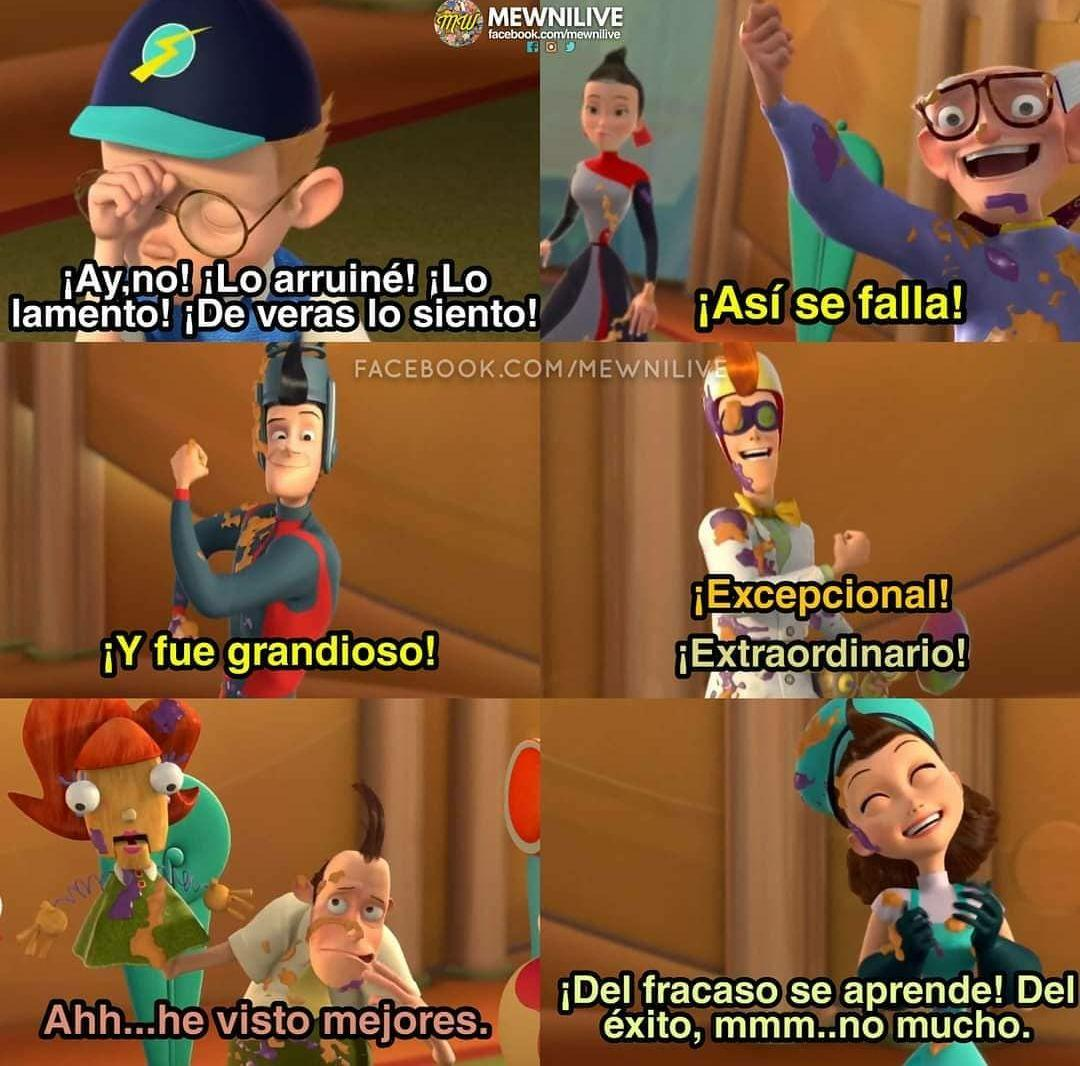
\includegraphics[width=0.52\textwidth]{./imagenes/familia.jpg}
\end{figure} 
\end{document}
